\documentclass[12pt,journal,compsoc,twoside]{IEEEtran}

\hyphenation{op-tical net-works semi-conduc-tor}
\usepackage{pdflscape}
\usepackage{rotating}
\usepackage{graphicx}
\usepackage{multirow}
\usepackage{dcolumn}
\usepackage{booktabs}
\usepackage{amsmath}

\setlength{\textfloatsep}{10pt plus 4pt minus 4pt}

\begin{document}

\title{The Chaotic Dynamics of Aquatic Interactions}
\author{John Wang}

\markboth{18.353 Final Project}%
{\textit{Chaotic Dynamics of Aquatic Interactions}}

\IEEEspecialpapernotice{18.353 Final Project}

\maketitle

\begin{abstract}
The preservation of natural ecosystems has become an increasingly important area of research. We examine the dynamics of the hammerhead shark (\textit{Sphyrna lewini}), cownose ray (\textit{Rhinoptera bonasus}), and bay scallop (\textit{Argopecten irradians}) populations. We estimate parameters of the system for the east coast of the United States, obtain analytical results concerning the general equations, and apply this knowledge to make policy recommendations that stabilize the ecosystem. We also show that without government intervention, the endangered hammerhead shark population will die off. 
\end{abstract}

\section{Introduction}

We consider the following ecosystem, where $X,Y,$ and $Z$ are the number of scallops, cownose rays, and hammerhead sharks respectively. We assume these populations evolve continuously as:
\begin{eqnarray}
\dot{X} &=& R_0 X(1 - X/K_0) - C_1 F_1(X) Y \nonumber \\
\dot{Y} &=& F_1 (X) Y - F_2 (Y) Z - D_1 Y \\
\dot{Z} &=& C_2 F_2(Y) Z - D_2 Z \nonumber \\
 F_i(U) &=& \frac{A_i U}{B_i + U} \nonumber
\end{eqnarray}

We can nondimensionalize the system using the following dimensionless variables:
\begin{eqnarray}
x &=& X/K_0 \nonumber \\
y &=& C_1 Y/ K_0 \nonumber \\
z &=& C_1 Z / (C_2 K_0) \\
t &=& R_0 T \nonumber
\end{eqnarray}

Which leads to the following nondimensionalized system:
\begin{eqnarray}
\dot{x} &=& x(1-x) - f_1(x) y \nonumber \\
\dot{y} &=& f_1(x) y - f_2(y) z - d_1 y \\
\dot{z} &=& f_2(y) z - d_2 z \nonumber \\
f_i(u) &=& \frac{a_i u}{1 + b_i u} \nonumber
\label{eqn:system}
\end{eqnarray}

\section{Parameter Fitting}

\subsection{Parameter Interpretations}

It is evident that $K_0$ represents the carrying capacity of the scallops, and $R_0$ represents the logistic growth rate of the population. The conversion factors $C_1$ and $C_2$ must have dimensions [scallops/rays] and [sharks/rays] in order for them to nondimensionalize $y$ and $z$. These parameters represent the carrying capacity of rays and sharks in terms of $K_0$. One can also see that $D_1$ is the death rate of a rays and $D_2$ is the death rate of sharks. 

Analyzing the functions $F_i$ show that they must have dimensions of [1/time]. This means that $A_i$ has units of [1/time] and $B_i$ has units of population. $A_i$ represents the frequency of predation in a unit of time, while $B_i$ represents a close to average population size. 

\subsection{Parameter Values}

In light of these observations, we can attempt to fit these parameter values to our problem. First, we will only consider the region where scallops and cownose rays are prominent, which is on the eastern coast of the United States. We will pick the area where scallops usually inhabit, which roughly corresponds to the coastline between North Carolina and Cape Cod. This is about 800 miles of coastline, and scallops inhabit up to about 3 miles offshore \cite{Fay(1983)}. Scallop densities in the late 1970s and early 1980s were about 20 scallops per square meter, which is historically close to the highest density reached \cite{Fay(1983)}. This means that we have a carrying capacity of roughly $K_0 = 1 \times 10^{11}$ scallops in our region. The average density of scallops now has dropped dramatically and is probably closer to 5 scallops per square meter, which leads to roughly $B_1 = 2 \times 10^{10}$. 

Next, we note that cownose rays consume about 1.5\% of their body weight each day according to \cite{Neer(2005)} who determines consumption based on $VO_2$ respiration. The average cownose ray weighs about 10kg while the average scallop weighs about 0.02kg. Thus, assuming scallops consist for about 50\% of a ray's diet, the average ray consumes about 1300 scallops per year. If we assume that cownose rays eat scallops five times a day, we have parameter values of roughly $A_1 = 5$ and $C_1 =380$. 

The average density of cownose rays in Chesepeake Bay is roughly 0.001 rays per square meter \cite{Blaylock(1993)}. We can estimate $C_1$ from this data as well. Assuming we have roughly a density of 2.5 scallops per square meter (since scallop densities dropped off dramatically since \cite{Fay(1983)} performed their measurements), we see that there are about $C_1 = 2.5/(0.001*5) = 500$ scallops per ray. Taking the average of the two $C_1$ values we obtained, we will use $C_1 =  440$. We can also obtain the parameter for the average population of rays $B_2 = 5 \times 10^{6}$ using this estimate.

Hammerhead sharks consume about 2\% of their body weight each day \cite{Bush(2002)}. Since hammerheads weigh about 150kg, and cownose rays are about 10kg, we see that hammerheads consume about 50 cownose rays per year if we assume cownose rays account for about 50\% of the hammerhead diet. Thus, we find the parameter values of $A_2 = 3$ and $ C_2 = 1/50 = 0.02$.  

Death rates can be obtained by looking at average lifetimes and assuming uniform distributions of age. Cownose rays live for about 15 years, so we obtain $D_1 = 0.07$, while hammerheads live about 25 years, so $D_2 = 0.04$. We assume a growth rate of $R_0 = 20$. 

\begin{table}[ht!]
\centering
\caption{\sffamily{Parameter Value Estimates}}
\setlength{\extrarowheight}{2pt}
\begin{tabular}{@{}>{\sffamily}l >{\sffamily}l >{\sffamily}l >{\sffamily}c >{\sffamily}c} 
\toprule[1.5pt]
 & Paremeter & Dimension & Value & References \\
\midrule
\multicolumn{5}{l}{\textbf{Dimensionless Conversion Parameters}} \\
&$C_1$ & [scallops/rays] & 440 & \cite{Neer(2005)} and \cite{Blaylock(1993)}\\
&$C_2$ & [sharks/rays] & 0.02 & \cite{Bush(2002)}\\
\\[-8pt]
\multicolumn{5}{l}{\textbf{$F_1$ and $F_2$ Function Parameters}} \\
&$A_1$ & [1/time] & 5 & \\
&$A_2$ & [rays/(time $*$ sharks)] & 3 & \\
&$B_1$ & [scallops] & $2 \times 10^{10}$ & \cite{Fay(1983)} \\
&$B_2$ & [rays] & $5 \times 10^{6}$ & \cite{Blaylock(1993)} \\
\\[-8pt]
\multicolumn{5}{l}{\textbf{Scallop Population Parameters}} \\
&$K_0$ & [scallops] & $1 \times 10^{11}$ & \cite{Fay(1983)} \\
&$R_0$ & [1/time] & 20 & \\
\\[-8pt]
\multicolumn{5}{l}{\textbf{Death Rates}} \\
&$D_1$ & [1/time] & 0.07 & \\
&$D_2$ & [1/time] & 0.04 & \\
\bottomrule[1.5pt]
\end{tabular}
\end{table}

\subsection{Dimensionless Parameters}

Since we have estimates for the parameters in our original equations, we can find the nondimensionalized parameters. We can express the nondimensionalized equations in terms of the dimensionalized coefficients. This is done by setting $\vec{x} = h(\vec{X})$, where $h$ is the function that maps $X,Y,Z$ to $x,y,z$. After we have $d\vec{x}/dt$ in terms of $\vec{X}$, we can collect terms and regroup $X,Y,Z$ into $x,y,z$ terms to obtain the following:
\begin{eqnarray}
\frac{dx}{dt} &=& \frac{dX}{dT} \frac{1}{K_0 R_0} \nonumber \\
&=& \frac{1}{K_0 R_0} \left( R_0 X \left(1 - \frac{X}{K_0} \right) - C_1 \frac{A_1 X}{B_1 + X} Y \right) \nonumber \\
&=& x(1-x) - \frac{\frac{A_1 K_0}{R_0 B_1} x}{1 + \frac{K_0}{B_1} x} y \\
\frac{dy}{dt} &=& \frac{dY}{dT} \frac{C_1}{R_0 K_0} \nonumber \\
&=& \frac{C_1}{R_0 K_0} \left( \frac{A_1 X}{B_1 + X} Y - \frac{A_2 Y}{B_2 + Y} Z - D_1 Y \right) \nonumber \\
&=& \frac{ \frac{A_1 K_0}{R_0 B_1} x}{1 + \frac{K_0}{B_1} x} y - \frac{\frac{A_2 K_0 C_2}{R_0 B_2 C_1}y}{1 + \frac{K_0}{B_2 C_1} y } z - \frac{D_1}{R_0} y \\
\frac{dz}{dt} &=& \frac{dZ}{dT} \frac{C_1}{R_0 C_2 K_0} \nonumber \\
&=& \frac{C_1}{R_0 C_2 K_0} \left( C_2 \frac{A_2 Y}{B_2 + Y} Z - D_2 Z \right) \nonumber \\
&=& \frac{ \frac{C_2 A_2 K_0}{R_0 B_2 C_1} y}{1 + \frac{ K_0}{B_2 C_1} y} z - \frac{D_2}{R_0} z  
\end{eqnarray}

Using these equations, we can obtain the expressions for the dimensionless parameters in terms of the parameters from the original equation. Using these expressions, we can obtain estimated values for $a_i, b_i$, and $d_i$ based on the estimated values for the parameters from the original equations. Substituting these values into the dimensionless equations, we have:
\begin{eqnarray}
\dot{x} &=& x(1-x) - \frac{x }{1 + 5 x}y \nonumber \\
\dot{y} &=& \frac{x}{1 + 5 x} y - \frac{0.1 y}{1 + 45 y} z - d_1 y \\
\dot{z} &=& \frac{0.1 y}{1 + 45 y} z - d_2 z \nonumber
\end{eqnarray}

\begin{table}[ht!]
\centering
\caption{\sffamily{Dimensionless Parameters}}
\label{table:dimensionless}
\setlength{\extrarowheight}{2pt}
\begin{tabular}{@{}>{\sffamily}l >{\sffamily}l >{\sffamily}l >{\sffamily}r } 
\toprule[1.5pt]
 & Parameter & Expression & Estimated Value  \\
\midrule
\multicolumn{4}{l}{\textbf{$F_1$ and $F_2$ Function Parameters}} \\
&$a_1$ & $\frac{A_1 K_0}{R_0 B_1}$ & 1 \\
&$a_2$ & $\frac{A_2 K_0 C_2}{R_0 B_2 C_1}$ & 0.1 \\
&$b_1$ & $\frac{K_0}{B_1}$ & 5  \\
&$b_2$ & $\frac{K_0}{B_2 C_1}$ & 45\\
\\[-8pt]
\multicolumn{4}{l}{\textbf{Death Rates}} \\
&$d_1$ & $\frac{D_1}{R_0}$ & $4 \times 10^{-3}$ \\
&$d_2$ & $\frac{D_2}{R_0}$ & $2 \times 10^{-3}$ \\
\bottomrule[1.5pt]
\end{tabular}
\end{table}

\section{Simple Properties}

\subsection{Fixed Points}
\label{sec:fixedpts}

The first analysis one can perform is to look for fixed points of the nondimensionalized system where $\frac{d}{dt}\vec{x} = 0$. A trivial fixed point is where $\vec{x}_1 = (0,0,0)$. To analyze its local stability, we can linearize and find the Jacobian of the system evaluated at $\vec{x}_1$. The Jacobian is:
%\begin{equation}
% \left[ \begin{array}{c c c}
%1 - 2x - \frac{a_1 y}{(1 + b_1 x)^2} & - \frac{a_1 x }{1 + b_1 x} & 0 \\
%\frac{a_1 y}{(1 + b_1 x)^2} & \frac{a_1 x}{1 + b_1 x} - \frac{a_2 z}{(1 + b_2 y)^2} - d1 & - \frac{a_2 y}{1 + b_2 y} \\
%0 & \frac{a_2 z}{(1 + b_2 y)^2} & \frac{a_2 y}{1 + b_2 y} - d_2 
%\end{array} \right]
%\end{equation}
\begin{equation}
\begin{bmatrix}
\left[1 - 2x - \frac{a_1 y}{(1 + b_1 x)^2}\right], \; \left[- \frac{a_1 x }{1 + b_1 x}\right], \; \left[0\right] \\
\left[\frac{a_1 y}{(1 + b_1 x)^2} \right], \; \left[\frac{a_1 x}{1 + b_1 x} - \frac{a_2 z}{(1 + b_2 y)^2} - d1 \right], \; \left[ - \frac{a_2 y}{1 + b_2 y} \right] \\
[0], \; \left[\frac{a_2 z}{(1 + b_2 y)^2} \right], \; \left[\frac{a_2 y}{1 + b_2 y} - d_2 \right] 
\end{bmatrix}
\end{equation}

Substituting $(x,y,z) = (0,0,0)$ into the Jacobian, we find:
\begin{equation}
J(0,0,0) = \left[ \begin{array}{c c c}
1 & 0 & 0 \\
0 & -d1 & 0 \\
0 & 0 & - d2
\end{array} \right]
\end{equation}

It is clear that the linearized equations decouple and we obtain $x(t) = x_0 e^t, y(t) = y_0 e^{-d_1 t},$ and $ z(t) = z_0 e^{-d_1 t}$. Since $d_1$ and $d_2$ are death rates which are always positive, we see that $y(t)$ and $z(t)$ decay to 0. However, the $x(t)$ equation grows with time. Physically, this means that small perturbations about the origin lead to the ray and shark populations dying out, while the scallop populations will increase and be repelled from the origin. This makes intuitive sense because small populations of all three animals means the predators will most likely die off, while the scallop population without predators should increase. 

The other fixed point that occurs for all parameters is $\vec{x}_2 = (1,0,0)$. The Jacobian at $\vec{x}_2$ is the following:
\begin{equation}
J(1,0,0) = \left[ \begin{array}{ c c c}
-1 & -\frac{a_1}{1 + b_1} & 0 \\
0 & \frac{a_1}{1 + b_1} - d_1 & 0 \\
0 & 0 & -d_2 
\end{array} \right]
\end{equation}

Notice that the Jacobian is upper triangular so that the eigenvalues lie on the diagonals. The fixed point is locally stable if all the eigenvalues are negative, which is equivalent to the condition that $a_1/(1 + b_1) < d_1$.  Also notice that the equations decouple, since one can solve explicitly for $z(t) = z_0 e^{-d_2 t}$ and $y(t) = y_0 e^{(a_1/(1 + b_1) - d_1) t}$. Using our parameter estimates, we find $a_1 / (1 + b_1) = 0.17 \not < 4 \times 10^{-3}$. Thus, the $\vec{x}_2$ fixed point in our regime is not locally stable. 

\subsection{The Coordinate Axes}

Any points starting with $x=0$ will continue to have $x=0$ throughout time. This is because $x$ can be factored out of the $\dot{x}$ equation, so that $\dot{x} = 0$ if $x = 0$. This holds for $y=0$ and $z=0$ as well. Thus, points beginning on any axis will stay on that axis throughout time because the $x=0$, $y=0$, and $z=0$ values cannot change. In addition, all trajectories beginning on the z-axis of $x=y=0$ move towards the origin, since the $z(t)$ equation decouples and becomes $z(t) = z_0 e^{-d_2 t}$. Similarly, points on the y-axis move towards the origin at $y(t) = y_0 e^{-d_1t}$. Points on the x-axis of $y=z=0$ follow logistic growth of $\dot{x} = x(1-x)$.  

Notice that the invariance of all three axes means that phase space is broken up into eight quadrants. Trajectories in one quadrant can never cross over into another quadrant. Since we are working with a physical system representing populations, we will remain in the first quadrant with $x, y, z \geq 0$. 

\subsection{Volume Contraction}

Unlike in the Lorenz equations, this system does not have volume contraction in general. However, there are certain regions for which volume contraction occurs. Using the divergence theorem, we can derive
\begin{equation}
\dot{V} = \int_V \nabla \vec{f} dV
\end{equation}

Volume contraction occurs for regions where $\nabla \vec{f} < 0$. We can compute this for our system:
\begin{eqnarray}
\nabla \vec{f} &=& 1 - d_1 - d_2 - 2x \nonumber \\
&+& \frac{a_1 (x - y)}{1 + b_1 x} + \frac{a_2 (y - z)}{1 + b_2 y} \nonumber \\
&+& \frac{a_1 b_1 x y}{(1 + b_1 x)^2} + \frac{a_2 b_2 y z}{(1 + b_2 y)^2}
\end{eqnarray}

There is at least one parameter regime for which there is volume contraction. If $1 < d_1 + d_2$:
\begin{equation} 
\lim_{b_1, b_2 \to \infty} \nabla \vec{f} = 1 - d_1 - d_2 - 2x < 0
\end{equation}

Thus, for very large values of $b_1$ and $b_2$, one can obtain volume contraction as long as $d_1 + d_2 > 1$ are large enough. In these parameter regimes, there are no quasiperiodic solutions.\footnote{If quasiperiodic solutions existed, then they would lie of the surface of some manifold whose volume is constant in time. But since there is volume contraction, this leads to a contradiction.}

\section{Limit Cycles and Attractors}

Numerical experiments suggest that there exists an attractor somewhere in the region about the origin, but only in the $xy$ plane. We will show analytically that this attracting region exists as long as $d_1 < a_1 / (1 + b_1)$. Notice that this is the same condition for the $\vec{x}_2 = (1,0,0)$ fixed point to be unstable. After the analysis, it will be clear that the local stability of the $\vec{x}_2$ fixed point will be governed by the appearance of the attracting region, so that the appearance of the limit cycle will correspond exactly with the change in stability of $\vec{x}_2$. 

We see the trajectory in figure \ref{attractor} has periodic oscillations in the $xy$ plane. It seems to be bounded by some boxed region about the origin. Let us define this region in $xy$ space as $[0,x_h] \times [0, y_h]$, where $x_h$ and $y_h$ are constant values of $x$ and $y$ respectively. Clearly, trajectories can't leave the region through the $x$ or $y$ axis because $x,y \geq 0$ by the physical limitations of the system, and because once $x=0$ ($y = 0$) then $x$ stays 0 forever (similarly with $y = 0$). Therefore, we need to make sure no trajectories leave from the vertical $x = x_h$ line and the horizontal $y = y_h$ line. 

On the vertical $x = x_h$ line, we need to check that $\dot{x} < 0$, so that trajectories only enter the region. We have:
\begin{equation}
\dot{x} = x_h(1 - x_h) - \frac{a_1 x_h}{1 + b_1 x_h} y
\end{equation}

The second term in this equation is always negative. The largest it can be is $0$ when $y = 0$. Thus, $x_h ( 1 - x_h) < 0$ is a sufficient condition for $\dot{x} < 0$. This implies that $x_h > 1$ will guarantee that trajectories only enter the region through the $x = x_h$ vertical line. 

On the horizontal line $y = y_h$, we need to check that $\dot{y} < 0$:
\begin{equation}
\dot{y} = \frac{a_1 x}{1 + b_1 x} y_h - \frac{a_2 y_h}{1 + b_2 y_h} z - d_1 y_h
\end{equation}

Clearly the second and third terms are always nonpositive. The second term's maximum occurs when $z = 0$. The coefficient of the first term $a_1 x / (1 + b_1 x)$ is an increasing function in $x$. We know that the maximum value of $x$ in the region is $x_h > 1$. Thus, the maximum value of the first term is $a_1 / (1 + b_1)$, and occurs when $x_h = 1$. Therefore, we see that $\dot{y} < 0$ exactly when:
\begin{equation}
\frac{a_1}{1 + b_1} > d_1
\end{equation}

Thus, there exists a trapping region $[0,x_h] \times [0, y_h]$ when $a_1 / (1 + b_1) > d_1$ (since the first condition $x_h > 1$ can always be satisfied). 

\subsection{Attractor Existence}
\label{sec:attractorexist}

Notice that there is a fixed point $\vec{x}_3 = (x^{*},y^{*},z^{*})$ that might exist inside the trapping region. This occurs at 
\begin{equation}
\vec{x}_3 = \left( \frac{d_1}{a_1 - b_1 d_1}, \frac{a_1 - d_1 - b_1 d_1}{(a_1 - b_1 d_1)^2}, 0 \right)
\end{equation}

The $a_1 / (1 + b1) > d_1$ condition guarantees that $a_1 > d_1 (1 + b_1)$ so that $y^{*} > 0$ when the trapping region exists, since the numerator $a_1 - d_1(1 + b_1) >0$ and the denominator $(a_1 - b_1 d_1)^2$ are always positive. Since we can choose any $y_h$ line for which $\dot{y} < 0$ given our condition of $a_1 > d_1 ( 1 + b_1)$, we can choose $y_h > y^{*}$. This means that the $y$ coordinate of $\vec{x}_3$ is inside the trapping region, so that $0 < y^{*} < y_h$.

To show that the $x^{*}$ coordinate must be inside the trapping region, we must have $a_1 > b_1 d_1$ for $x^{*} > 0$. This follows directly from the $a_1 - d_1(1 + b_1) > 0$ condition, since $a_1 - b_1 d_1 > d_1$ and $d_1 \geq 0$, so that $a_1 - b_1 d_1 > 0$. Moreover, since $a_1 - b_1 d_1 > d_1$, we see that $x^{*} = d_1 / (a_1 - b_1 d_1) < 1 = x_h$. Therefore $0 < x^{*} < x_h$, which means the $x$ coordinate of $\vec{x}_3$ must lie in the trapping region if it exists. Thus if the trapping region exists, then the fixed point $\vec{x}_3$ will always exist in the trapping region. 

It is difficult to analytically examine stability of $\vec{x}_3$, since the Jacobian evaluated at $\vec{x}_3$ gives a complicated expression. However, we can make qualitative observations. If $\vec{x}_3$ is unstable and we have parameters such that no other fixed point exists in the trapping region, then there must be some type of attracting manifold. This follows because all trajectories flow into the trapping region, but never settle down to any fixed point.

Moreover, we can say something even stronger if $\vec{x}_3$ has positive eigenvalues corresponding to the $x$ and $y$ coordinates. This would mean $\vec{x}_3$ is a repeller in the $x$ and $y$ coordinates, so that one can construct a circle of radius $\epsilon$ about the fixed point in the $xy$ plane and show that all trajectories are driven outside this circle. By Poincar\'{e} Bendixson, a limit cycle must exist in the $xy$ plane. Note, however, that this is not a limit cycle in phase space, since we only gauranteed a degenerate limit cycle in a 2 dimensional subspace. \footnote{If one plotted the $x$ and $y$ coordinates against each other, one would see a limit cycle. This corresponds to looking down onto the $xy$ plane from some $z > 0$}

\subsection{Example System with Attracting Manifold}

Using certain parameters, we can show there exists some attracting manifold inside the $xy$ trapping region. Take $b_1 = 5, b_2 = 45, a_2 = 0.1, d_2 = 0.002$ like before, but now change $d_1 = 2$ and $a_1 = 25$. This corresponds to a regime where fishing of rays increases dramatically. Our analysis has shown that a trapping region should exist when $a_1 / (1 + b_1) > d_1$, which is indeed the case since $a_1 ( 1 + b_1) = 25 / 6 > d_1 = 2$. Moreover, one can numerically solve for the Jacobian at $\vec{x}_3 = (0.13, 0.06, 0)$. The eigenvalues of the linearized system are $0.11 \pm 1.0i$ and $-4.0 \times 10^{-4}$. The real parts of the complex eigenvalues are positive and shows that the fixed point at $\vec{x}_3$ is unstable. Moreover, one can numerically show that the other fixed points with real, nonnegative values are $\vec{x}_1 = (0,0,0)$ and  $\vec{x}_2 = (1,0,0)$. Thus, $\vec{x}_3$ is the only fixed point that lies inside the trapping region. Since it is unstable, our analysis in section \ref{sec:attractorexist} shows that we should see an attracting manifold and limit cycle in the $xy$ plane.

\begin{figure}[h]
\centering
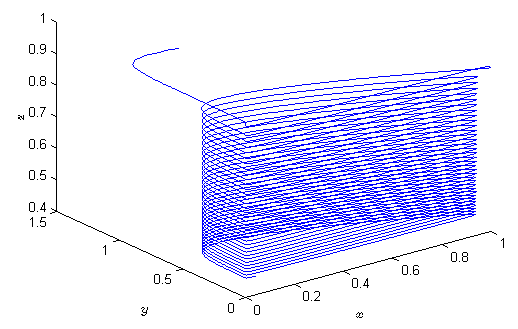
\includegraphics[width=2.5in, trim = 10 20 10 20]{attractor.png}
\caption{Cylindrical Attractor}
\label{attractor}
\end{figure}

Indeed, this is the case. Figure \ref{attractor} shows a trajectory entering the trapping region given these parameters. Rotating the figure to look down onto the $xy$ plane shows a stable limit cycle. Changing the $d_1$ parameter to $a_1 ( 1 + b_1) + 0.01$ eliminates the manifold, as seen in figure \ref{noattractor}, although one can see a ghost of the cylindrical shape in the trajectories.

\begin{figure}[h!]
\centering
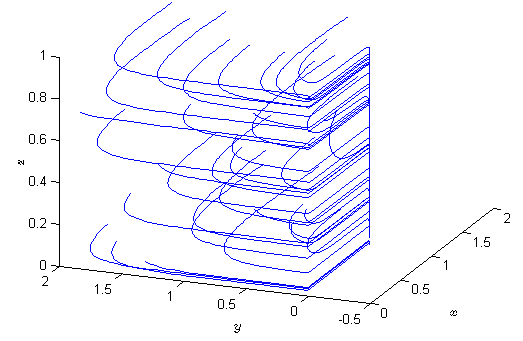
\includegraphics[width=2.5in, trim = 10 20 10 20]{noattractor.png}
\caption{Ghost of Cylindrical Attractor}
\label{noattractor}
\end{figure}

\subsection{Pear Shaped Trajectories}
\label{sec:pear}

In some instances, trajectories take interesting paths before reaching a limit cycle. Figure \ref{pear} shows a trajectory tracing out a pear shaped object before arriving at a limit cycle in the upper right corner of the figure. The figure is drawn with the following system: $d_1 = 0.03, d_2 = 0.001, a_1 = 2, a_2 = 0.01, b_1 = 1, b_2 = 1$. Since $a_1 / (1 + b_1) = 1 < d_1 = 0.03$, our analytical results predict an attracting manifold. 

\begin{figure}[h!]
\centering
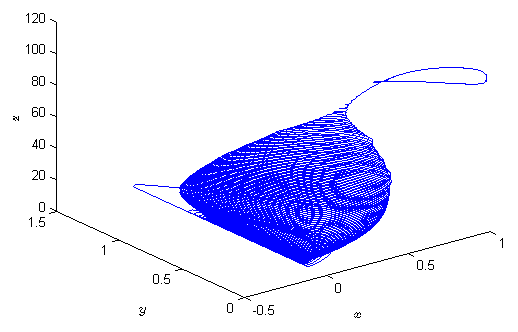
\includegraphics[width=2.5in, trim = 10 20 10 20]{pear.png}
\caption{Pear Shaped Trajectory with Limit Cycle}
\label{pear}
\end{figure}

Fixed point analysis shows that in addition to $(0,0,0),(1,0,0)$, and $\vec{x}_3 = (0.015, 0.50, 0)$, we have another real, nonnegative fixed point at $\vec{x}_4 = (0.88, 0.11, 100)$. The two fixed points $\vec{x}_3$ and $\vec{x}_4$ lie in the trapping region. The Jacobian about $\vec{x}_3$ has eigenvalues of $-2.6 \times 10^{-4} \pm 0.17i$ and $2.3 \times 10^{-3}$. Although this fixed point is stable in the $xy$ plane, it is unstable in general. The other fixed point at $\vec{x}_4$ has eigenvalues of $0.86, -7.9,$ and $9.7 \times 10^{-4}$. Thus, this fixed point is also unstable and we find two unstable fixed points in the trapping region. The pear shape is centered about the $\vec{x}_3$ fixed point. The trajectory then climbs upwards around the pear until it reaches the region surrounding the $\vec{x}_4$ fixed point. 

\begin{figure}[h!]
\centering
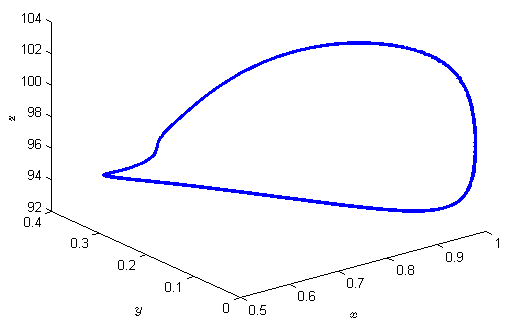
\includegraphics[width=2in, trim = 10 20 10 20]{limitcycle.png}
\caption{Limit Cycle About $\vec{x}_4$}
\label{limitcycle}
\end{figure}

We can show numerically that the trajectory surrounding the $\vec{x}_4$ fixed point is probably a limit cycle. Figure \ref{limitcycle} shows a close up of the trajectory in the upper right corner of figure \ref{pear}. It is a closed orbit that repeats itself with period of about $P = 140$. 

\section{Chaotic Attracting Manifolds}

Although they can arise in the trapping region, limit cycles are not guaranteed. There exist other attracting manifolds which do not lead to periodic orbits. Consider the following parameter regime: $d_1 = 0.03, d_2 = 0.014, a_1 = 1.3, a_2 = 0.1, b_1 = 3,$ and $b_2 = 1$. An attracting manifold exists because $a_1 / (1 + b_1) = 0.325 > d_1 = 0.03$, and the trajectory in figure \ref{chaoscycle} shows a portion of this attractor. 

\begin{figure}[h!]
\centering
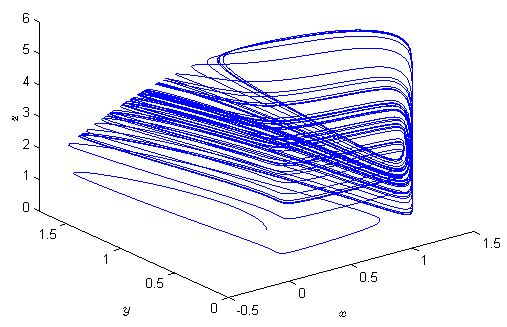
\includegraphics[width=2.5in, trim = 10 20 10 20]{chaoscycle.png}
\caption{Chaotic Attracting Manifold}
\label{chaoscycle}
\end{figure}

The variation of the $x$ coordinate throughout time in figure \ref{chaosxt} does not seem to be periodic. Altough the trajectory appears to repeat itself, just like in the Lorenz Attractor, these periodic regimes seem to differ slightly. None of these periods are exactly aligned, and it is clear from figure \ref{chaoscycle} that trajectories do not intersect and settle down to a stable equilibrium.

\begin{figure}[h!]
\centering
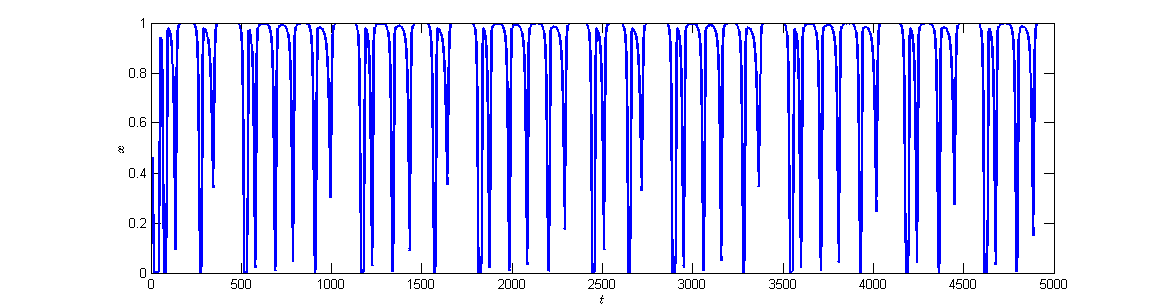
\includegraphics[width = 3in, trim = 10 20 10 20]{chaosxt.png}
\caption{Trajectory of $x(t)$ Throughout Time}
\label{chaosxt}
\end{figure}

\subsection{One Dimensional Map}

Figure \ref{chaosxt} shows apparently chaotic behavior, but this may eventually settle down to a periodic solution after a long enough time period. To get a better sense of this behavior, one can build a map of the local minima of $x(t)$, where $x_{n+1} = f(x_n)$ is given by the $x$ value of the next local minimum after $x_n$. 

\begin{figure}[h!]
\centering
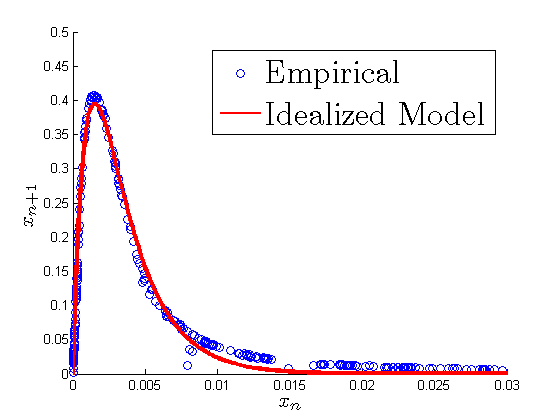
\includegraphics[width = 2.5in, trim = 10 20 10 20]{map.png}
\caption{Local Minima Map}
\label{map}
\end{figure}

The map looks like a log-normal distribution. However, the log-normal distribution is difficult to examine analytically. Therefore, we will simplify the empirical distribution using an idealized model. We can approximate the shape in figure \ref{map} using $c_1, c_2, c_3$ and $c_4$ as undetermined positive constants in the relationship:
\begin{equation}
x_{n+1} = f(x_n) = c_1 e^{c_2 x} + c_3 e^{c_4 x}
\end{equation}

The idealized model in figure \ref{map} uses $c_1 = -1.12, c_2 = -1100, c_3 = 1.1,$ and $c_3 = -390$. 

\subsection{Fixed Points and Stability}

The fixed points occur when $x_{n+1} = x_{n} = x^{*}$. For our parameters, this fixed point occurs $x^{*} = 1.84 \times 10^{-5}$. To examine its stability, we shall take its derivative and check $|f'(x^{*})|$. We have
\begin{equation}
f'(x^{*}) = c_2 c_1 e^{c_2 x^*} + c_4 c_3 e^{c_4 x^*}
\end{equation}

Evaluating, we find $|f'(x^{*})| \approx 3050$, so the fixed point is unstable. We can also look at fixed points for $f_2(x) = f(f(x))$, which correspond to double period fixed points, or $f_3(x) = f(f(f(x)))$ which correspond to triple period fixed points. In general, we have the following recursive relationship between the derivative of $f_{n-1}$ and $f_{n}$:
\begin{eqnarray}
f_n'(x^{*}) &=& \left( c_1 c_2 e^{c_2 f_{n-1}(x^{*})} \right. \nonumber \\
&+& \left. c_3 c_4 e^{c_4 f_{n-1}(x^{*})} \right) f_{n-1}'(x^{*}) \nonumber \\ 
&=& f_1'(f_{n-1}(x^*)) f_{n-1}'(x^*) 
\label{eqn:recursion}
\end{eqnarray}

By following the recursion, we can rewrite equation \ref{eqn:recursion} into the following:
\begin{equation}
f_n'(x^*) = f_1 '(f_{n-1}(x^*)) \ldots f_1 '(f_2(x^*)) f_1 '(x^*) 
\end{equation}

Which can be further simplified into
\begin{equation}
f_n'(x^*) = f_1'(x^*) \prod_{i = 1}^{n-1} f_1 '(f_i (x^*))
\label{eqn:fnderiv}
\end{equation} 

To look at stability of fixed points, we must find when $|f_n'(x^*)| < 1$. Since equation \ref{eqn:fnderiv} is expressed completely in terms of $f_1'(t)$, we should analyze $f_1'(t)$ for the range of $t$ for which $|f_1'(t)| < 1$. This occurs for $t > 0.01$ and $t \approx 0.0015$. The region around $\hat{t} = 0.0015$ for which $|f_1'(\hat{t})| < 1$ is small enough that the effective region for which $|f_1'(t)| < 1$ is when $t > 0.01$. We can be almost sure that the $n$th period fixed point is unstable if all terms in equation \ref{eqn:fnderiv} have magnitude greater than 1. This means we have the following criterion for instability of all fixed points, given a fixed point $x^*$ of $f_n(x)$ :
\begin{equation}
f_i(x^*) < 0.01 \hspace{0.2cm} \forall i \in \{1,\ldots,n\} 
\end{equation}

To examine this numerically, we can note that stable fixed points for the $i$th period will also be stable fixed points for the $j$th period, where $i < j$. Thus, if we cannot find stable fixed points in the $j$th period, where $j >> 1$, then it is unlikely that stable fixed points exist at all. We take a large $j = 200$ and calculate $f_{200}(x_k) = x_{k+1}$ for $2000$ iterations. Figure \ref{fptransient} shows the last 400 iterations of this calculation. There is no block of 200 points which repeats itself in the last $400$ iterations, which shows that $f_{200}(x)$ (and subsequently all $f_i(x)$ for $i < 200$) probably does not have a stable fixed point. 

\begin{figure}[h!]
\centering
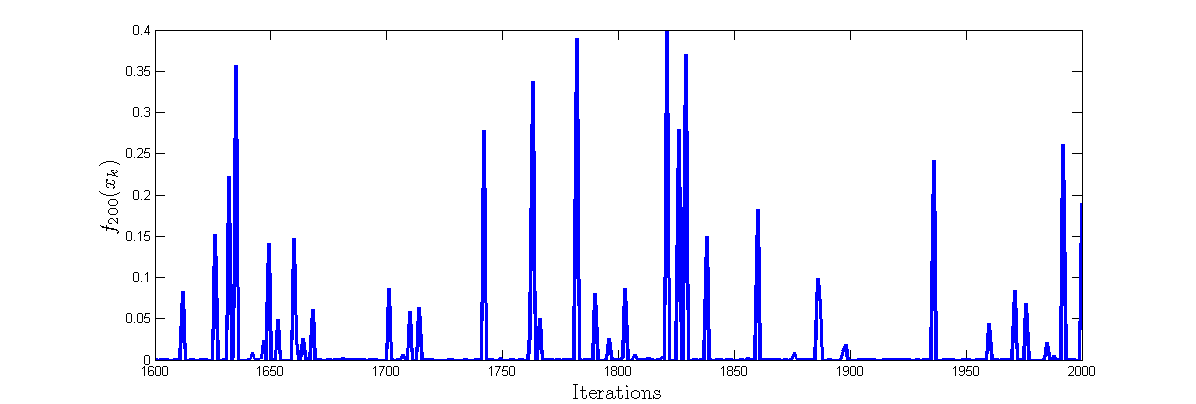
\includegraphics[width=3.5in]{fptransient.png}
\caption{Last 400 Iterations of $f_{200}(x_k)$}
\label{fptransient}
\end{figure}

It seems unlikely that a completely different pattern would arise for extremely large $j$ and contradict previous evidence of unstable fixed points. However, if stable solutions of period $j > 200$ do exist, these solutions would show transient chaos and would seem chaotic for all practical purposes.  

%\subsection{Dependence on Initial Conditions}
%
%We have shown that trajectories in the current regime are both apreriodic and determininstic. In order for us to label this chaos, we must also have sensitive dependence on initial conditions. 

\subsection{Fractal Dimension of Manifold}

One can compute the fractal dimension of the manifold in figure \ref{chaoscycle} by using the correlation dimension. We compute a trajectory for a long period of time (almost all trajectories on an attractor have the same long term statistics, so a single trajectory is sufficient). Let $N_{x}(\epsilon)$ be the number of points lying within a ball of radius $\epsilon$ centered about a point $x$ on the trajectory. Now let $C(\epsilon) = ( \sum_{i = 1}^{k} N_{x_i}(\epsilon) ) / k$ be the average of $N_x (\epsilon)$ over many points of $x$. We should have the following relationship:
\begin{equation}
C(\epsilon) \propto \epsilon^d
\end{equation}

Where $d$ is the correlation dimesion. A modified version of the Grassberger-Procaccia Algorithm was implemented in Matlab. First, it was tested on the Lorenz Attractor, and found a dimension of 2.19, which is reasonably close to dimension of 2.05 found by Grassberger and Procaccia originally. 
\begin{figure}[h!]
\centering
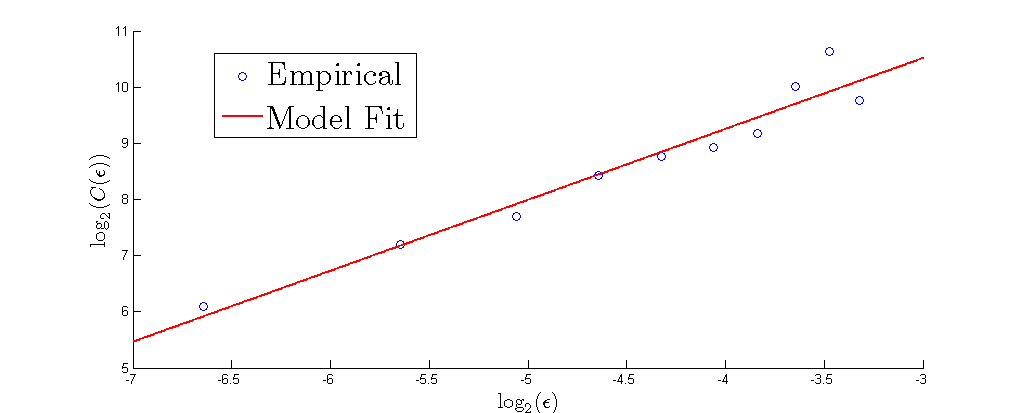
\includegraphics[width=3in]{fractaldimen.png}
\caption{Grassberger-Procaccia  Results}
\label{fractaldimen}
\end{figure}

The algorithm was run on the system in figure \ref{chaoscycle} using a random set of initial conditions within the cube $[0,1] \times [0,1] \times [0,1]$. A total of $5 \times 10^{5}$ iterations were computed, with the first $1 \times 10^{5}$ being discarded to make sure the trajectory reached the attractor. For each $\epsilon$ in the set $\bigcup_{i = 1}^{20} \{0.01 i \}$, $N_x(\epsilon)$ was averaged over 100 randomly chosen points on the attractor.  Figure \ref{fractaldimen} shows the results of the calculation. The $x$ axis shows $\log_2(\epsilon)$ while the $y$ axis shows $\log_2(C(\epsilon))$. The fitted linear model gives a slope of $1.38 \pm 0.09$.  

Thus, the fractal dimension of the attractor in figure \ref{chaoscycle} is $d = 1.38$. At first glance, this dimension seems incorrect since the shape in figure \ref{chaoscycle} seems three dimensional. However, after running the algorithm five more times with different ranges of $\epsilon$, we find that $d = 1.38$ is relatively robust. A possible explanation of this phenomenon is that the attracting manifold is never completely covered by a trajectory. Much like trying to cover a ball with a piece of yarn, figure \ref{chaoscycle} shows that there exist sizeable gaps between nearby parts of the trajectory. Although figure \ref{chaoscycle} shows $t$ up to $t = 1.5 \times 10^{4}$, increasing the length of integration to $t = 7.5 \times 10^{4}$ does not change the qualitative observation that there are gaps between nearby parts of the trajectory.   

To show that simply increasing the length of integration would not change this result, the calculation in figure $\ref{fractaldimen}$ was performed again with $5 \times 10^{6}$ iterations (an order of magnitude larger than before), and run for a smaller set of $\epsilon$ in $\bigcup_{i=1}^{10} \{ 0.001i \}$. The empirical model yielded $d = 1.46$, which is within the 95\% confidence interval of our first estimate. This evidence suggests that the fractal dimension of the manifold is indeed close to $d = 1.38$. 

\section{Policy Recommendations}

With a solid theoretical underpinning, we can begin to analyze the system in equation \ref{eqn:system} with our estimated parameters. First, we examine the natural course of events.

\subsection{Natural Ecosystem}

In the natural ecosystem with parameters from table \ref{table:dimensionless}, we see that almost all trajectories settle down to an attracting manifold. Figure \ref{naturaleco} shows the 3D phase portrait of the system with a variety of initial conditions. Each of the trajectories quickly moves onto an attracting manifold which almost touches the $x$ axis and the trajectories spend most of their time near $x = 0$. 

\begin{figure}[h!]
\centering
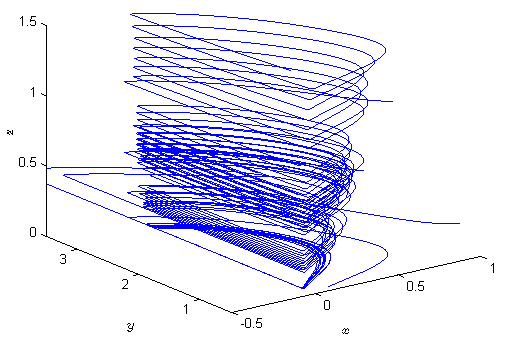
\includegraphics[width=2.5in]{naturaleco.png}
\caption{Phase Portrait of Natural Ecosystem }
\label{naturaleco}
\end{figure}

The shark population ($z$ coordinate) is mostly stable, while the $y$ coordinate has a slow decay towards zero before it jumps back to a higher level. The $x$ and $y$ coordinates have behavior reminiscent of a relaxation oscillation, as shown in figure \ref{naturalecoxy}. The $x$ coordinate stays below 0.001 for about 400 time steps until it suddenly spikes upwards. The $y$ coordinate decays to about 75\% of its previous maximum until the relxation phase, when it jumps back close to its previous maximum again. The process repeats itself about every 400 time steps.  

\begin{figure}[h!]
\centering
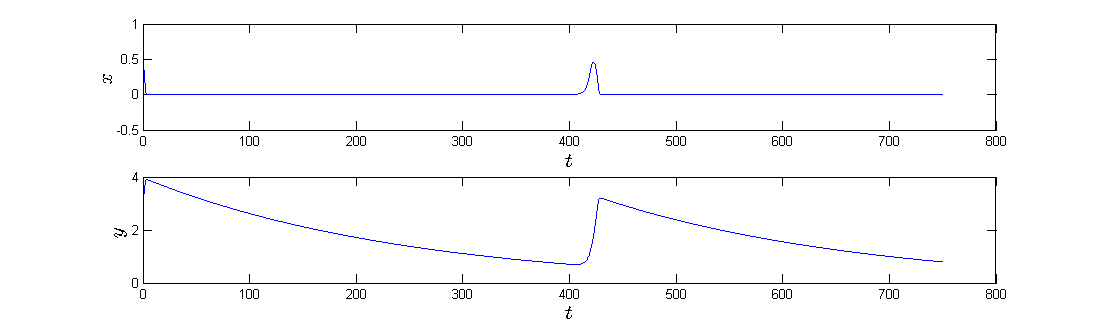
\includegraphics[width=3.5in]{naturalecoxy.png}
\caption{Natural $x(t)$ and $y(t)$ Trajectories}
\label{naturalecoxy}
\end{figure}

The relaxation oscillation has implications for the natural growth of aquatic populations. In particular, it means that the scallops will stay almost nonexistent for long periods of time, and have short outbursts of population. The rays will steadily die off, until the short outbursts of the scallop population rejuvenate the ray population. The shark population will stay mostly constant.

These long term dynamics suggests that the natural ecosystem may not lead to the best economic solution, since the scallop fishing industry will most likely be devastated. 

\subsubsection{Parameter Testing}

However, it is possible that the parameters in table \ref{table:dimensionless} do not accurately represent the natural system parameters. This situation seems likely since we estimated these parameters with large degrees of uncertainty. One parameter which seems rather uncertain in the nondimensionalized system is $b_2$, which is very large compared to the other parameters. We can plot the long term values of $x$ for different values of $b_2$. Figure \ref{longtermxt} plots $x(t)$ for $t \in [500,1000]$ on the $y$ axis.    
\begin{figure}[h!]
\centering
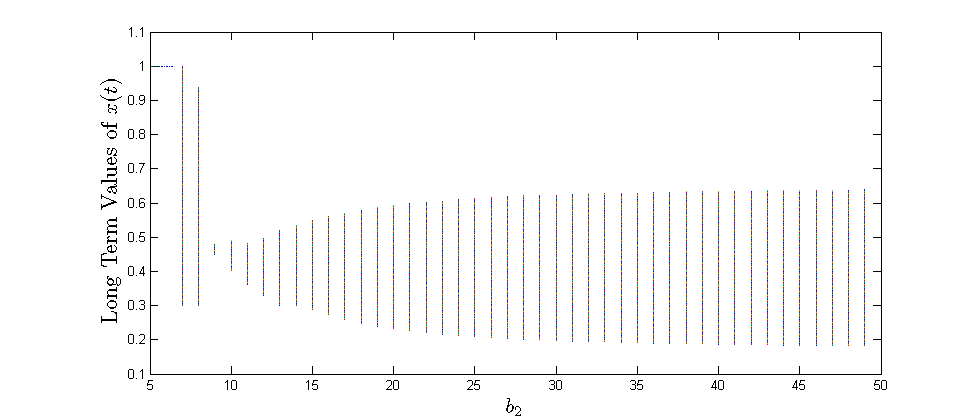
\includegraphics[width=3.5in]{longtermxt.png}
\caption{Long Term $x(t)$ Values}
\label{longtermxt}
\end{figure}

Figure \ref{longtermxt} shows that the long term behavior of $x(t)$ settles down for approximately $b_2 > 20$. Thus, we can be reasonably sure that our analysis is correct for the range of $b_2 > 20$. If our estimates are off by more than a factor of 2, however, then the natural ecosystem regime might be different.  

\subsubsection{Fishing of Sharks}

Now consider what happens when we account for the overfishing of sharks which has occurred in the recent years. Here, $d_2$ will increase since the death rate of sharks ($D_2$ in the original model) increases. This change on $d_2$, however, does not have drastic effects on the dynamics of the system. The sharks will, of course, tend to die off faster. The dynamics of the scallops and the rays, however, remains largely unchanged. This occurs because $b_2 = 45$ is high enough in comparison to $a_2 = 0.1$ that $f_2(y) = a_2 y / (1 + b_2 y)$ is relatively small for any value of $y$ in $[0,5]$. This means that the change in ray population due to predation by sharks will be relatively small (this is the $-f_2(y) z$ term in the second equation of \ref{eqn:system}) since $y$ rarely gets larger than 5.
\begin{figure}[h!]
\centering
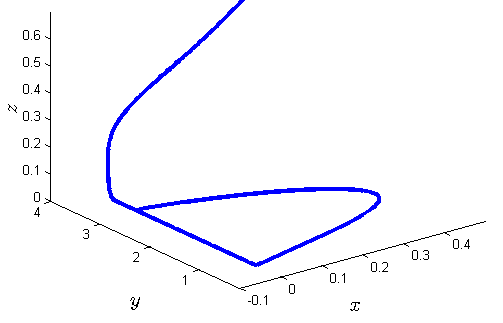
\includegraphics[width=2.5in]{sharkdeath.png}
\caption{Shark Death with $d_2 = 0.5$}
\label{sharkdeath}
\end{figure}

Indeed, figure \ref{sharkdeath} shows that the dynamics of the scallop and ray relaxation oscillations remain the same, but that the sharks die off. Here, we have changed $d_2 = 0.5$, but the figure is representative of $d_2$ in the approximate parameter range of $d_2 > 9 \times 10^{-3}$. The relaxation oscillation in the $x$ and $y$ values occurs on the parabolic loop of the $xy$ plane. Thus, the introduction of shark fishing does not produce drastic changes in the ecosystem in general because of the small number of sharks with respect to rays. In effect, the shark population can be thought of as independent of the ray population because $b_2 >> a_2$ in the natural ecosystem.

\subsection{Fishing of Rays}

What if the government instituted a policy of fishing rays? Could this help save the shark population and the scalloping industry? Recall that parameters with $a_1 / (1 + b_1) > d_1$ led to the existence of an attracting manifold. Both the natural ecosystem and the ecosystem with shark overfishing have an attracting manifold because $a_1 / (1 + b_1) = 0.17 >  0.004 = d_1$. Thus, changing $d_1$ to any parameter value below 0.17 will most likely lead to previously found regimes (which were unsatisfactory). For instance, take $d_1 = 0.08$ and $d_2 = 0.02$. Here, we have stayed in the regime with relaxation oscillations in the scallop and ray populations, but we also have a decaying shark population. Figure \ref{doublefishing} shows the decay of the shark population as the scallop and ray populations oscillate. 
\begin{figure}[h!]
\centering
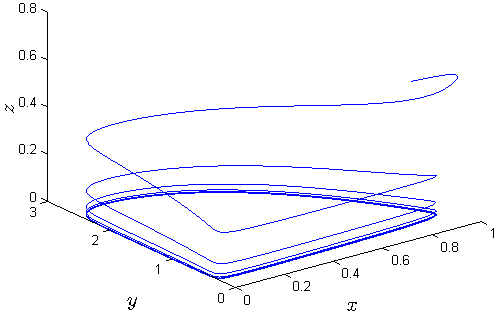
\includegraphics[width=2.5in]{doublefishing.png}
\caption{Mild Fishing of Both Sharks and Rays}
\label{doublefishing}
\end{figure}

Thus, we must attempt to exhaust our options and find regimes without attracting manifolds, testing whether these lead to healthy aquatic populations. Unfortunately, once we exit the regime of attracting manifolds and set $d_1 > 0.16$, $\vec{x}_2 = (1,0,0)$ becomes a stable fixed point (recall from section \ref{sec:fixedpts} that once $a_1/(1 + b_1) < d_1$, then all eigenvalues of $\vec{x}_2$ become negative, so that $\vec{x}_2$ becomes stable). Figure \ref{stablex2} shows 50 trajectories with different initial conditions settling down to the $\vec{x}_2$ fixed point. 
\begin{figure}[h!]
\centering
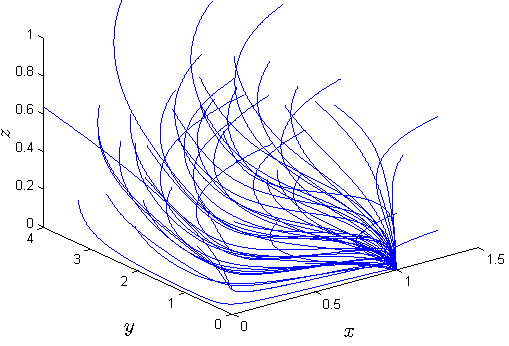
\includegraphics[width=2.5in]{stablex2.png}
\caption{Stability of $x_2 = (1,0,0)$}
\label{stablex2}
\end{figure}

Thus, even though $\vec{x}_2$ is only locally stable, it seems that most trajectories starting out with reasonable initial conditions tend to settle down to $\vec{x}_2$.\footnote{Reasonable here means that initial conditions begin inside the $[0,2] \times [0,2] \times [0,2]$ cube in $\mathrm{R}^3$.} Since both shark and ray populations die out at $\vec{x}_2$, the fishing of rays does not seem like a good government solution.

\subsection{Ban on Shark Fishing}

Another possible solution is a government ban on shark fishing, which would correspond to setting $d_2 = 0$. However, this solution will cause some undesired results in terms of the ray population. This is because the sharks will grow wildly and feed on the ray population until the rays die off to extremely low levels and only scallops and sharks are left.
\begin{figure}[h!]
\centering
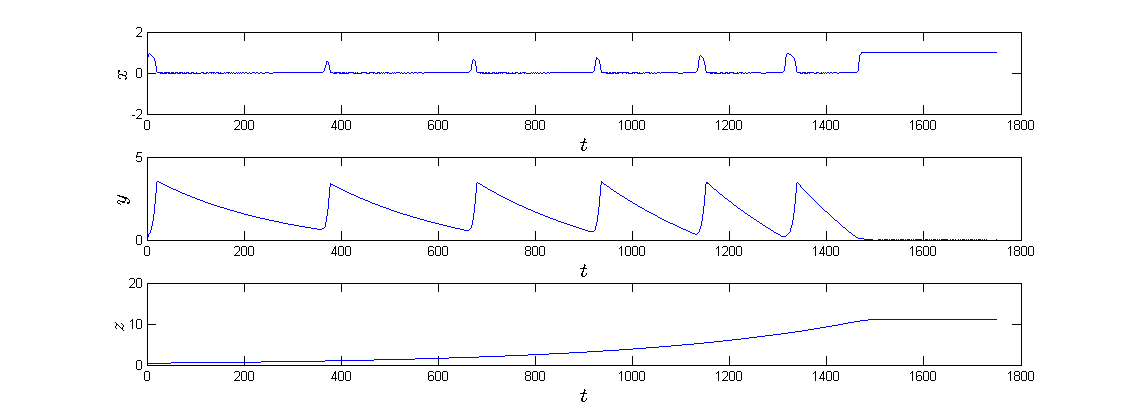
\includegraphics[width=3.55in]{bansharkfishing.png}
\caption{Populations After Shark Fishing Ban}
\label{bansharkfishing}
\end{figure}

Figure \ref{bansharkfishing} shows the $x(t), y(t)$ and $z(t)$ trajectories for $t \in [0, 1750]$ when $d_2 = 0$ in our original system. At first, relaxation oscillations occur for scallop and ray populations. However, the shark population eventually grows large enough so that $y(t)$ stays at essentially 0 as $t \to \infty$. This solution is not satisfactory either. 

\subsection{Pear Shaped Trajectories}

Since none of the other solutions have worked, we shall go back and rely on the knowledge we have previously derived. Recall that the pear shaped trajectory in section \ref{sec:pear} had a stable limit cycle that oscillated about a real, nonnegative fixed point. Since all $x,y,$ and $z$ coordinates on this limit cycle were positive, this would correspond to a stable oscillatory regime where each aquatic population stayed alive indefinitely.

Thus, the government can attempt to coerce the current parameters into a regime with a pear shaped trajectory. The pear shaped trajectory would create a stable limit cycle and keep each aquatic population at a healthy level. To minimize the number of parameters that must be changed, we will look for a pear shaped trajectory that most closely matches the parameters of the natural ecosystem.
\begin{figure}[h!]
\centering
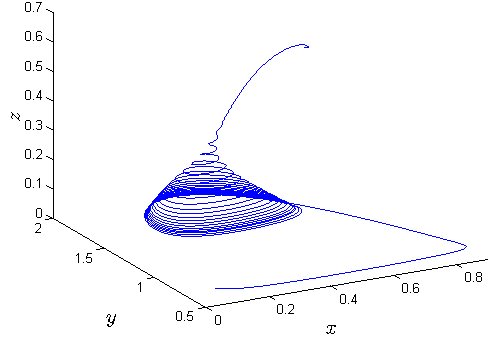
\includegraphics[width=2.5in]{pear2.png}
\caption{Pear Shaped Trajectory with Stable Fixed Point}
\label{pear2}
\end{figure}

A pear shaped regime can be found by changing the following parameters: $b_2 = 1, d_1 = 0.13, d_2 = 0.06$, with the other parameters remaining the same. A trajectory in 3D phase space is given figure \ref{pear2}, with dynamics similar to those seen in figure \ref{pear}. A large number of oscillations with small $z$ eventually lead to a stable point with a positive $z$ coordinate.  
\begin{figure}[h!]
\centering
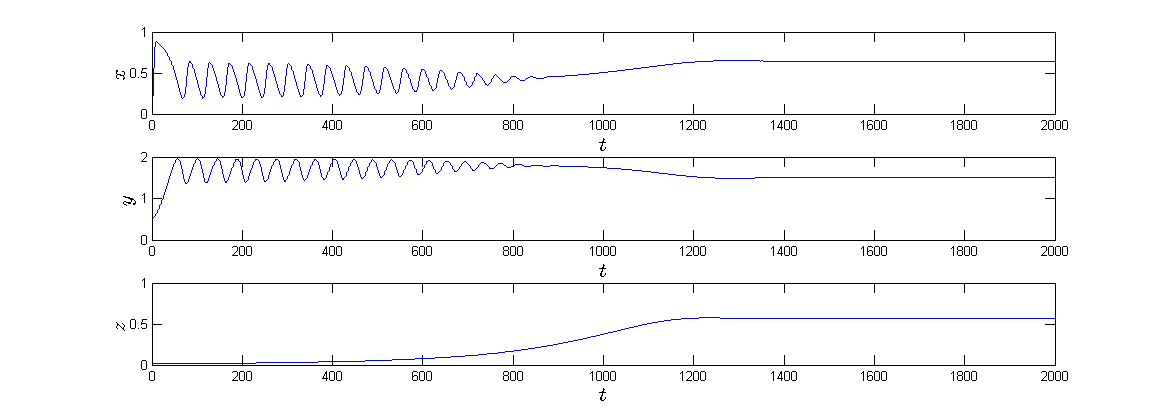
\includegraphics[width=3.55in]{peartrajectory.png}
\caption{Pear Shaped Trajectories in Time}
\label{peartrajectory}
\end{figure}

Figure \ref{peartrajectory} shows that the $x(t),y(t),$ and $z(t)$ coordinates eventually settle down to a stable fixed point at $\vec{x}_p = (0.64, 1.5, 0.57)$ as $t \to \infty$. Thus, this parameter regime actually settles down to become a stable ecosystem. Even better, the parameter changes from $d_1 = 0.004 \to {d_1}_p = 0.13$ and $d_2 = 0.002 \to {d_2}_p = 0.06$ can be easily obtained by allowing more fishing of rays and sharks. Not only is it easy to allow this, but the citizens may actually support the government's increase of shark fishing.

The hardest parameter to change will be $b_2 = 45 \to {{b_2}_p} = 1$. Recall that in terms of our original parameters, we have $b_2 = K_0 / (B_2 C_1)$. Thus, the government can either attempt to increase $B_2$ or $C_1$, or attempt to decrease $K_0$. All of these actions will have consequences on $a_2 = (A_2 K_0 C_2) / (R_0 B_2 C_1)$. However, since $C_1$ and $C_2$ only appear in $a_2$ and $b_2$, one can adjust both $C_2$ and $C_1$ in order to decrease $b_2$ while keeping $a_2$ constant. The government needs to increase $C_2$ by the exact same amount as $C_1$. This is difficult, however, since $C_1$ and $C_2$ represent the carrying capacity of scallops and sharks respectively in terms of rays. 

However, this seems like the best chance for the government which has exhausted all other easy policy solutions. Let us call this the ``Pear Policy'' and examine how the government can implement it.

\subsubsection{Implementation of the Pear Policy}

The government must decrease the natural carrying capacity of both scallops and sharks in comparison to rays. Notice that fishing alone will not be sufficient to implement the Pear Policy, since fishing does not affect natural carrying capacities. The government needs a solution that will limit the scallop and shark population in the absence of fishing.

One way to accomplish this is to fish other prey populations. Since sharks do not solely feed on rays, one can decrease the shark carrying capacity with respect to rays by limiting the shark population's other food supplies. For instance, the fishing of squid and octopus (two other fishes in the hammerhead diet) would likely decrease $C_2$. Constraining the main food supply of scallops (plankton) would likely decrease $C_1$. 

This approach, however, seems ill-advised. Since we have not modelled a system including the squid and octopus populations, we have no idea whether fishing will cause dramatic effects on other parts of the ecosystem. More importantly, we do not know how fishing will impact the squid or shark populations. It could be the case that some complicated dynamics lead to completely conterintuitive results and increase $C_2$ instead of decreasing it. We have shown in this paper that blindly applying guesses to a potentially chaotic system can lead to catastrophic results. Likewise, killing off the plankton population will almost certainly have consequences in the larger ecosystem, since plankton are basic sources of food for many aquatic animals.

This does not bode well for the survival of the scallop, ray, and shark ecosystem. The ecosystem's demise results mainly from the difficulty of arriving at a stable fixed point or limit cycle by changing natural parameters. Instead, one could let the natural ecosystem run its course, but protect the shark population in a autonomous system (for example in fisheries).

\subsection{Fisheries}

If the government removed all sharks from the ecosystem and allowed them to live in a fishery with an abundant supply of food, then the natural shark population would reach $z = 0$. Thus, we have a new two dimensional set of equations:
\begin{eqnarray}
\dot{x} &=& x(1-x) - f_1(x)y \nonumber \\
\dot{y} &=& f_1(x) y - d_1 y 
\end{eqnarray}

Where $f_1(x) = a_1 x /(1+ b_1 x)$ is defined as before. We can leave the population parameters the same at $a_1 = 1, a_2 = 0.1, b_1 = 5$, and $b_2 = 45$ (of course $a_2$ and $b_2$ no longer matter here). One could then increase $d_1$ (the fishing of rays) to some value below $a_1 / (1 + b_1) = 1/6$ to induce a stable attracting manifold about positive $x$ and $y$ populations. This would result in the following trajectories with $d_1 = 0.13$:
\begin{figure}[h!]
\centering
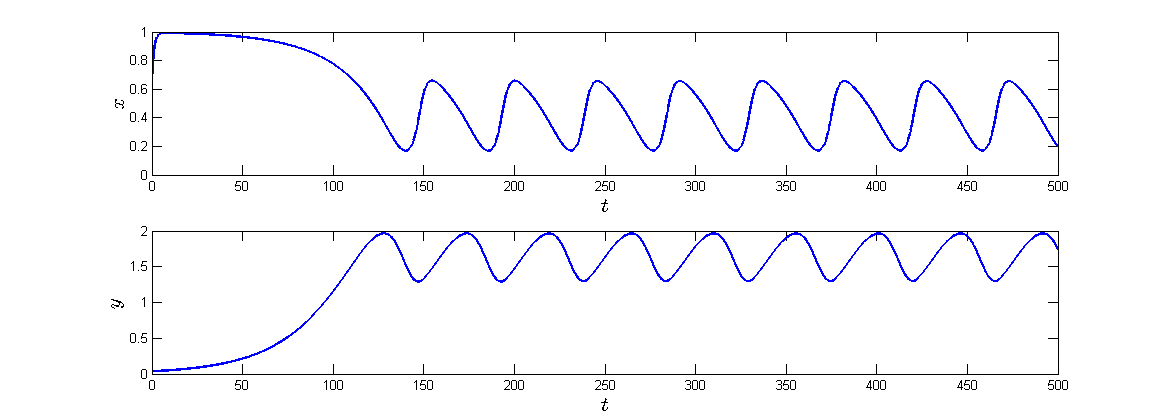
\includegraphics[width=3.5in]{success.png}
\caption{Stable Oscillations in Scallop and Ray Populations}
\label{success}
\end{figure}

Thus, we can solve our ecosystem problem by fishing rays and creating a fishery for the hammerhead sharks. Although this does not give the government a cost-effective solution, it will keep the scallop, ray, and shark populations alive indefinitely. In fact, the government could tax the scallop fishing industry (which would have been devastated in the natural ecosystem) to pay for the shark fishery. 

\section{Conclusion}

This paper has analyzed an ecosystem of scallops, rays, and hammerhead sharks. We conclude that the natural ecosystem without fishing leads to the economic collapse of the scallop fishing industry, while the fishing of sharks leads to the death of the shark population. The government's best solution is to create a shark fishery and allow for the fishing of rays. 

\bibliographystyle{acm}
\bibliography{bibliography}
\nocite{*}

\end{document}


